\documentclass[11pt,a4paper]{article}

\usepackage[utf8]{inputenc}
\usepackage[T1]{fontenc}
\usepackage{lmodern}
\usepackage[margin=2.4cm]{geometry}
\usepackage{amsmath,amssymb}
\usepackage{booktabs}
\usepackage{graphicx}
\usepackage{float}
\usepackage{array}
\usepackage{listings}
\usepackage{xcolor}
\usepackage[hidelinks]{hyperref}

\lstset{
  basicstyle=\ttfamily\small,
  backgroundcolor=\color{gray!8},
  frame=single,
  breaklines=true,
  columns=fullflexible
}

\renewcommand{\contentsname}{Daftar Isi}
\renewcommand{\figurename}{Gambar}
\renewcommand{\tablename}{Tabel}
\renewcommand{\refname}{Daftar Pustaka}

\begin{document}

\begin{titlepage}
\centering
\vspace*{1.5cm}
{\large\textbf{LAPORAN TEKNIS PROYEK AKHIR HIGH PERFORMANCE COMPUTING}\par}
\vspace{1.2cm}
{\LARGE\bfseries Implementasi dan Evaluasi Ring Attention dengan Blockwise Transformer pada Mesin Multi-core Menggunakan OpenMP dan MPI\par}
\vspace{0.5cm}
{\Large\itshape Studi Kasus: Triase Cepat Sampel Sekuens DNA Jaringan Payudara\par}
\vspace{1.8cm}

\begin{tabular}{llp{7.2cm}}
\toprule
\textbf{Nama Anggota} & \textbf{NIM} & \textbf{Peran Utama (Proposal Bagian 9)} \\
\midrule
Dhimas Early Oceandy & \texttt{24/533508/PA/22584} & V0 (FP32 \& FP64), V1, pipeline tokenisasi 6-mer, pelatihan offline PyTorch \\
Mahardika Ramadhana & \texttt{24/538247/PA/22831} & Kernel GEMM ter-tile, Online Softmax per tile, V2 OpenMP, V4 Hybrid MPI+OpenMP \\
Thufail Bahir Al Bariq & \texttt{24/537843/PA/22801} & V3 Ring Attention MPI, integrasi inferensi C++, koordinator repositori \\
Kevin Febriano & \texttt{24/541948/PA/23002} & Mikro-benchmark ($F, B$), skrip eksperimen, visualisasi, demo, dan analisis \\
\bottomrule
\end{tabular}

\vfill
{\large
Program Studi Ilmu Komputer\\
Departemen Ilmu Komputer dan Elektronika\\
Fakultas Matematika dan Ilmu Pengetahuan Alam\\
Universitas Gadjah Mada\\
November 2026
\par}
\end{titlepage}

\begin{abstract}
Mekanisme \emph{self-attention} standar pada arsitektur Transformer memerlukan materialisasi matriks skor $S = QK^\top / \sqrt{d} \in \mathbb{R}^{s \times s}$ yang tumbuh kuadratik $\mathcal{O}(s^2)$ terhadap panjang sekuens $s$, sehingga membatasi panjang konteks pada perangkat komputasi tunggal. Laporan ini menyajikan implementasi, verifikasi numerik, dan evaluasi kinerja \textbf{Ring Attention} berbasis \emph{Blockwise Transformer} dan \emph{Online Softmax} pada satu mesin multi-core tanpa GPU melalui emulasi proses MPI dan thread OpenMP. Kami membangun empat versi inti secara bertahap (\textbf{V0} \emph{naive} FP64 acuan dan FP32 $\mathcal{O}(s^2)$, \textbf{V1} \emph{blockwise serial}, \textbf{V2} \emph{blockwise} OpenMP, dan \textbf{V3} \emph{Ring Attention} MPI dengan rotasi \emph{double buffer} \texttt{[K|V]}) ditambah ekstensi opsional \textbf{V4} (hibrida MPI + OpenMP), serta menerapkannya pada studi kasus triase cepat sampel sekuens DNA jaringan payudara (\textit{BioProject PRJNA913438}).

Seluruh versi memakai kernel komputasi FP32 yang seragam (GEMM \emph{cache-blocked} $48 \times 64 \times 64$ dengan \emph{micro-kernel} AVX2/FMA $6 \times 16$ hingga \texttt{47.795 GFLOP/s} pada satu core) dan menghasilkan galat relatif $L_2$ terhadap acuan FP64 sebesar \texttt{3.24e-07}--\texttt{3.31e-07} pada input $\mathcal{N}(0,1)$ serta \texttt{1.225e-06}--\texttt{1.227e-06} pada uji stres logit besar $\mathcal{N}(0,10^2)$. Profil memori membuktikan \emph{delta RSS} per proses pada \textbf{V3} konstan di kisaran \texttt{4.288}--\texttt{4.588 KiB} untuk $c=2048$ ($s \in \{2048, 4096, 8192\}$)---61,5$\times$ lebih kecil daripada \textbf{V0} (\texttt{270.436 KiB}) pada $s=8192$. Di bawah pembatasan memori virtual \texttt{ulimit -v 1200000} KiB pada $s=16384$, \textbf{V0} gagal \texttt{std::bad\_alloc}, sedangkan \textbf{V3} ($P=4, c=4096$) sukses dalam \texttt{1.23435 s} dengan \emph{delta RSS} \texttt{11.616 KiB}. Pada $s=4096, d=64, P=4$, \textbf{V2} dan \textbf{V3} mencapai percepatan \texttt{4.194x} dan \texttt{4.098x}, uji \emph{overlap} mencapai $\eta = 0.8106$ di $c=2048$, dan aplikasi triase DNA ($s=8192$) dipercepat \texttt{2.94x}--\texttt{3.17x} dengan penghematan memori aktivasi lebih dari 42$\times$.
\end{abstract}

\tableofcontents
\newpage

\section{Pendahuluan dan Studi Kasus Bioinformatika (\texorpdfstring{\texttt{PRJNA913438}}{PRJNA913438})}

\subsection{Latar Belakang Memori Kuadratik dan Ring Attention}
Mekanisme \emph{scaled dot-product self-attention} \cite{vaswani2017} didefinisikan sebagai
\begin{equation}
\mathrm{Attention}(Q, K, V) = \mathrm{softmax}\!\left(\frac{Q K^\top}{\sqrt{d}}\right) V, \qquad Q, K, V \in \mathbb{R}^{s \times d}.
\end{equation}
Materialisasi penuh matriks skor $S \in \mathbb{R}^{s \times s}$ menuntut $\mathcal{O}(s^2)$ memori: pada presisi FP32 ($w=4$ byte), $s=16384$ memakan $1\text{ GiB}$ hanya untuk matriks skor. Teknik \emph{Online Softmax} \cite{milakov2018} dan komputasi per blok \cite{dao2022,liu2023bpt} menghitung softmax secara eksak tanpa menyimpan matriks $S$ penuh. Untuk pasangan blok query $Q_i \in \mathbb{R}^{c \times d}$ dan blok KV $(K_j, V_j) \in \mathbb{R}^{c \times d}$, statistik berjalan per baris $(m, \ell, O_i)$ diperbarui sebagai:
\begin{align}
m^{\mathrm{new}} &= \max\!\left(m^{\mathrm{old}}, \max_{\mathrm{col}}(S_{ij})\right), &
\alpha &= \exp\!\left(m^{\mathrm{old}} - m^{\mathrm{new}}\right), \\
P_{ij} &= \exp\!\left(S_{ij} - m^{\mathrm{new}}\right), &
\ell^{\mathrm{new}} &= \alpha \ell^{\mathrm{old}} + \sum_{\mathrm{col}} P_{ij}, \\
O_i^{\mathrm{new}} &= \alpha O_i^{\mathrm{old}} + P_{ij} V_j, &
O_i^{\mathrm{final}} &= \frac{O_i}{\ell}.
\end{align}
Sifat \emph{permutation invariance} pada penggabungan statistik ini mendasari \textbf{Ring Attention} \cite{liu2023ring}: setiap rank MPI $r$ menyimpan $Q_r$ tetap, sedangkan blok $[K|V]$ dirotasi sepanjang cincin perangkat sambil menumpangtindihkan (\emph{overlap}) komunikasi non-blocking dengan komputasi blok.

\subsection{Rumusan Masalah dan Tujuan}
Proyek ini menjawab empat pertanyaan inti: (1) validitas numerik \emph{Online Softmax} blockwise terhadap acuan FP64; (2) pembuktian memori per proses $\mathcal{O}(cd)$ independen terhadap $s$; (3) efektivitas \emph{overlap} komunikasi--komputasi ($\eta$), skalabilitas \emph{strong/weak scaling}, serta validasi model analitik $c \ge 2F/B$ pada mesin multi-core; dan (4) peningkatan latensi, \emph{throughput}, memori, serta panjang konteks maksimum $s$ pada aplikasi triase sekuens DNA.

\subsection{Studi Kasus DNA Jaringan Payudara (\texttt{PRJNA913438})}
Dataset \textit{whole-genome sequencing} (WGS) sel epitel payudara manusia (HMEC, BioProject \texttt{PRJNA913438}) \cite{park2023} berisi 779 juta hingga 1,008 miliar read ($\sim 150\text{ bp}$) pada satu lini normal pra-stasis (\texttt{184D}) dan tujuh lini seri progresi karsinogenesis (\texttt{184A1}, \texttt{184AA4}, \texttt{184B5}, \texttt{184AA2}, \texttt{184AA3}, \texttt{184B5ME}, \texttt{184FMY2}). Model Transformer berperan sebagai alat bantu triase awal (\texttt{Normal-like} vs \texttt{Progresi Karsinogenesis}) pada laboratorium kecil tanpa GPU.

\textbf{Keterbatasan Data:} Dataset asal hanya memiliki satu sampel normal (\texttt{184D}) dari satu spesimen; hasilnya tidak dapat digeneralisasi sebagai diagnosis klinis. Selain itu, karena \emph{SRA Toolkit} tidak tersedia di mesin lokal dan demi reproduksibilitas penuh tanpa unduhan puluhan GB, evaluasi memakai generator FASTQ sintetis offline (\texttt{--generate-synthetic-fastq}, 1.500 read/sampel = 37.500 token per lini untuk \texttt{184D}, \texttt{184A1}, \texttt{184B5}, \texttt{184AA2}), sementara opsi \texttt{--download-sra} tetap disediakan di skrip.

\section{Arsitektur Sistem dan Implementasi (V0--V4)}

\subsection{Pipeline End-to-End Aplikasi Triase DNA}
\begin{enumerate}
  \item \textbf{Tokenisasi 6-mer (\texttt{scripts/download\_and\_tokenize.py}):} Read $150\text{ bp}$ ditokenisasi non-overlapping ($k=6$, 25 token/read) dengan kosakata $4^6=4096$ ditambah \texttt{<UNK>=4096} dan \texttt{<PAD>=4097} (total 4098) menjadi biner \texttt{int32} di \texttt{data/tokens/}.
  \item \textbf{Pelatihan Offline PyTorch (\texttt{scripts/train\_offline\_pytorch.py}):} Arsitektur \texttt{BreastTriageTransformer} ($d=64$, 1 lapisan \emph{single-head attention} tanpa \emph{positional encoding} absolut, \emph{mean pooling}, dan linear classifier 2 kelas) dilatih di CPU pada konteks pendek $s_{\mathrm{train}}=512$ dan diekspor dalam FP32 \emph{row-major} ke \texttt{models/breast\_triage\_d64/}.
  \item \textbf{Inferensi C++/MPI (\texttt{src/inference/dna\_triage.cpp}):} Biner terpadu \texttt{./build/attn} menjalankan \emph{embedding lookup}, proyeksi $Q,K,V,O$ via \texttt{gemm\_nt\_fp32}, \emph{attention} (V0--V4), dan \emph{global mean pooling} melalui \texttt{MPI\_Allreduce} untuk V3/V4.
\end{enumerate}

\subsection{Kernel Bersama (\texttt{src/common/}) dan Desain V0--V4}
Seluruh versi V0--V4 memakai kernel bersama pada \texttt{src/common/gemm.cpp} (\texttt{gemm\_nt\_fp32} dan \texttt{gemm\_nn\_fp32}) yang menerapkan \emph{cache blocking} $48 \times 64 \times 64$ (muat di cache L1d $32\text{ KiB}$) dengan \emph{micro-kernel} AVX2+FMA $6 \times 16$, semantik \texttt{beta == 0.0f} bebas \texttt{NaN/Inf}, dan opsi \texttt{-DUSE\_OPENBLAS} (\texttt{OPENBLAS\_NUM\_THREADS=1}). Primitif \texttt{attend\_block\_online\_softmax} memproses tile internal $b_q \times b_k = 64 \times 64$ (scratchpad $16\text{ KiB}$ per thread).

\begin{table}[H]
\centering
\caption{Ringkasan implementasi versi V0 hingga V4.}
\begin{tabular}{llp{8.2cm}l}
\toprule
\textbf{Versi} & \textbf{Direktori} & \textbf{Mekanisme Paralelisme \& Komunikasi} & \textbf{Memori/Proses} \\
\midrule
V0 & \texttt{src/v0\_naive/} & Baseline naif FP64 acuan \& FP32 dengan materialisasi $S \in \mathbb{R}^{s \times s}$ & $\mathcal{O}(sd + s^2)$ \\
V1 & \texttt{src/v1\_blockwise/} & Serial \emph{blockwise} + \emph{Online Softmax} per tile $64\times 64$ & $\mathcal{O}(sd + c + b_q b_k)$ \\
V2 & \texttt{src/v2\_openmp/} & \texttt{\#pragma omp parallel for} di loop luar blok query (\emph{disjoint writes} ke $O$, buffer state privat per thread) & $\mathcal{O}(sd + P_{\mathrm{thr}} b_q b_k)$ \\
V3 & \texttt{src/v3\_ring\_mpi/} & Ring MPI dengan \emph{double buffer} gabungan \texttt{[K|V]} ($2cd$): mode \texttt{NonBlocking} (\texttt{Isend/Irecv}), \texttt{Blocking} (\texttt{Sendrecv}), dan \texttt{NoComm} & $\mathcal{O}(cd + b_q b_k)$ \\
V4 & \texttt{src/v4\_hybrid/} & Hibrida MPI Ring antar-rank + OpenMP sub-blok intra-rank (\texttt{MPI\_THREAD\_FUNNELED}, semua panggilan MPI di luar blok paralel) & $\mathcal{O}(cd + P_{\mathrm{thr}} b_q b_k)$ \\
\bottomrule
\end{tabular}
\end{table}

\section{Lingkungan Eksperimen dan Reproduksibilitas}

\begin{table}[H]
\centering
\caption{Spesifikasi perangkat keras dan perangkat lunak mesin eksperimen.}
\begin{tabular}{ll}
\toprule
\textbf{Komponen} & \textbf{Spesifikasi Terukur} \\
\midrule
CPU (Model) & Intel(R) Core(TM) i7-8665U CPU @ 1.90GHz (AVX2, FMA) \\
Core Fisik / Thread Logis & 4 core fisik / 8 thread logis \\
Cache L1d / L2 / L3 & 4 $\times$ 32 KiB / 4 $\times$ 256 KiB / 8 MiB shared \\
RAM & 15 GiB \\
Sistem Operasi & Ubuntu 24.04.5 LTS (\texttt{Linux 7.0.0-43-generic x86\_64}) \\
Kompilator & \texttt{g++} (GCC \texttt{13.3.0-6ubuntu2\textasciitilde 24.04.1}) \\
MPI & Open MPI \texttt{4.1.6} (\texttt{mpicxx}, \texttt{mpirun}) \\
Kernel BLAS & Kernel internal \texttt{tiled\_avx2\_fma} (\texttt{-O3 -march=native -fopenmp}, tanpa \texttt{-ffast-math}) \\
Lingkungan Python & Python \texttt{3.12.3}, NumPy \texttt{1.26.4}, Matplotlib \texttt{3.10.8}, PyTorch \texttt{2.14.1+cpu}, Streamlit \texttt{1.56.0} \\
\bottomrule
\end{tabular}
\end{table}

Seluruh pengujian mengikat proses/thread ke core fisik (\texttt{OPENBLAS\_NUM\_THREADS=1}, \texttt{OMP\_PROC\_BIND=close}, \texttt{OMP\_PLACES=cores}, \texttt{mpirun --bind-to core}) dengan minimal 5 pengulangan per konfigurasi. Karena \texttt{kernel.perf\_event\_paranoid = 4} membatasi \texttt{perf stat}, profiling dilakukan via \texttt{/usr/bin/time -v} serta mikro-benchmark GEMM dan ping-pong MPI.

\section{Hasil Eksperimen dan Analisis Mendalam}

\subsection{Verifikasi Kebenaran Numerik dan Uji Stres Logit}
Pada unit test mandiri, \texttt{test\_gemm} lolos 15/15 kasus (\texttt{rel\_l2 <= 1.48e-07}), \texttt{test\_v2\_openmp} lolos 10/10 kasus (termasuk kesamaan \emph{bit-exact} antar $P=1,2,4$), dan \texttt{test\_v4\_hybrid} lolos 6/6 kasus (\texttt{rel\_l2 <= 3.690e-06}). Tabel~\ref{tab:accuracy} merangkum verifikasi dari \texttt{results/raw/exp\_accuracy.csv} terhadap ground truth \textbf{V0-FP64} pada $s=1024, d=64, \text{tile}=64$.

\begin{table}[H]
\centering
\caption{Verifikasi numerik V0--V4 terhadap V0-FP64 (\texttt{exp\_accuracy.csv}).}
\label{tab:accuracy}
\begin{tabular}{lrrlrrl}
\toprule
\textbf{Versi} & \textbf{$P$} & \textbf{Threads} & \textbf{Skenario} & \textbf{Max Abs Err} & \textbf{Rel $L_2$ Err} & \textbf{Status} \\
\midrule
\texttt{v0} & 1 & 1 & \texttt{standard\_normal} & 1.991459e-07 & 3.241110e-07 & PASS \\
\texttt{v1} & 1 & 1 & \texttt{standard\_normal} & 2.373691e-07 & 3.310406e-07 & PASS \\
\texttt{v2} & 1 & 4 & \texttt{standard\_normal} & 2.373691e-07 & 3.310406e-07 & PASS \\
\texttt{v3} & 4 & 1 & \texttt{standard\_normal} & 2.140470e-07 & 3.300648e-07 & PASS \\
\texttt{v4} & 2 & 2 & \texttt{standard\_normal} & 2.373691e-07 & 3.305159e-07 & PASS \\
\texttt{v0} & 1 & 1 & \texttt{stress\_logits\_std10} & 1.529166e-05 & 1.226062e-06 & PASS \\
\texttt{v1} & 1 & 1 & \texttt{stress\_logits\_std10} & 1.514264e-05 & 1.225613e-06 & PASS \\
\texttt{v2} & 1 & 4 & \texttt{stress\_logits\_std10} & 1.514264e-05 & 1.225613e-06 & PASS \\
\texttt{v3} & 4 & 1 & \texttt{stress\_logits\_std10} & 1.505324e-05 & 1.225405e-06 & PASS \\
\texttt{v4} & 2 & 2 & \texttt{stress\_logits\_std10} & 1.514264e-05 & 1.226915e-06 & PASS \\
\bottomrule
\end{tabular}
\end{table}

Selain itu, paritas probabilitas PyTorch terhadap inferensi C++ (\textbf{V0} dan \textbf{V3}) pada $s=1024$ tercatat di bawah $4.30 \times 10^{-20}$.

\subsection{Analisis Memori per Proses dan Uji Batas \texorpdfstring{\texttt{ulimit -v}}{ulimit -v}}
Tabel~\ref{tab:memory} dan Gambar~\ref{fig:mem} memperlihatkan pertumbuhan memori kuadratik pada \textbf{V0} dibanding konstan $\mathcal{O}(cd)$ pada \textbf{V3} (\texttt{exp\_memory.csv}).

\begin{table}[H]
\centering
\caption{Profil memori per proses V0 vs V3 pada $c$ tetap (\texttt{exp\_memory.csv}).}
\label{tab:memory}
\begin{tabular}{llrrrrrrr}
\toprule
\textbf{Seri} & \textbf{Versi} & \textbf{$P$} & \textbf{$c$} & \textbf{$s$} & \textbf{Peak RSS (KiB)} & \textbf{Delta RSS (KiB)} & \textbf{Alloc Teoretis (KiB)} & \textbf{Waktu (s)} \\
\midrule
\texttt{v0\_naive} & \texttt{v0} & 1 & 1024 & 1024 & 178112 & 5388 & 5120.00 & 1.783724e-02 \\
\texttt{v0\_naive} & \texttt{v0} & 1 & 2048 & 2048 & 191332 & 18756 & 18432.00 & 6.918469e-02 \\
\texttt{v0\_naive} & \texttt{v0} & 1 & 4096 & 4096 & 242436 & 69848 & 69632.00 & 2.890142e-01 \\
\texttt{v0\_naive} & \texttt{v0} & 1 & 8192 & 8192 & 443212 & 270436 & 270336.00 & 1.862869e+00 \\
\texttt{v3\_c1024} & \texttt{v3} & 1 & 1024 & 1024 & 174872 & 2212 & 1560.00 & 1.633829e-02 \\
\texttt{v3\_c1024} & \texttt{v3} & 2 & 1024 & 2048 & 175316 & 2516 & 1560.00 & 3.359131e-02 \\
\texttt{v3\_c1024} & \texttt{v3} & 4 & 1024 & 4096 & 175280 & 2428 & 1560.00 & 6.992726e-02 \\
\texttt{v3\_c2048} & \texttt{v3} & 1 & 2048 & 2048 & 176832 & 4288 & 3104.00 & 6.696719e-02 \\
\texttt{v3\_c2048} & \texttt{v3} & 2 & 2048 & 4096 & 177336 & 4588 & 3104.00 & 1.321040e-01 \\
\texttt{v3\_c2048} & \texttt{v3} & 4 & 2048 & 8192 & 177232 & 4400 & 3104.00 & 2.805341e-01 \\
\bottomrule
\end{tabular}
\end{table}

\begin{figure}[H]
\centering
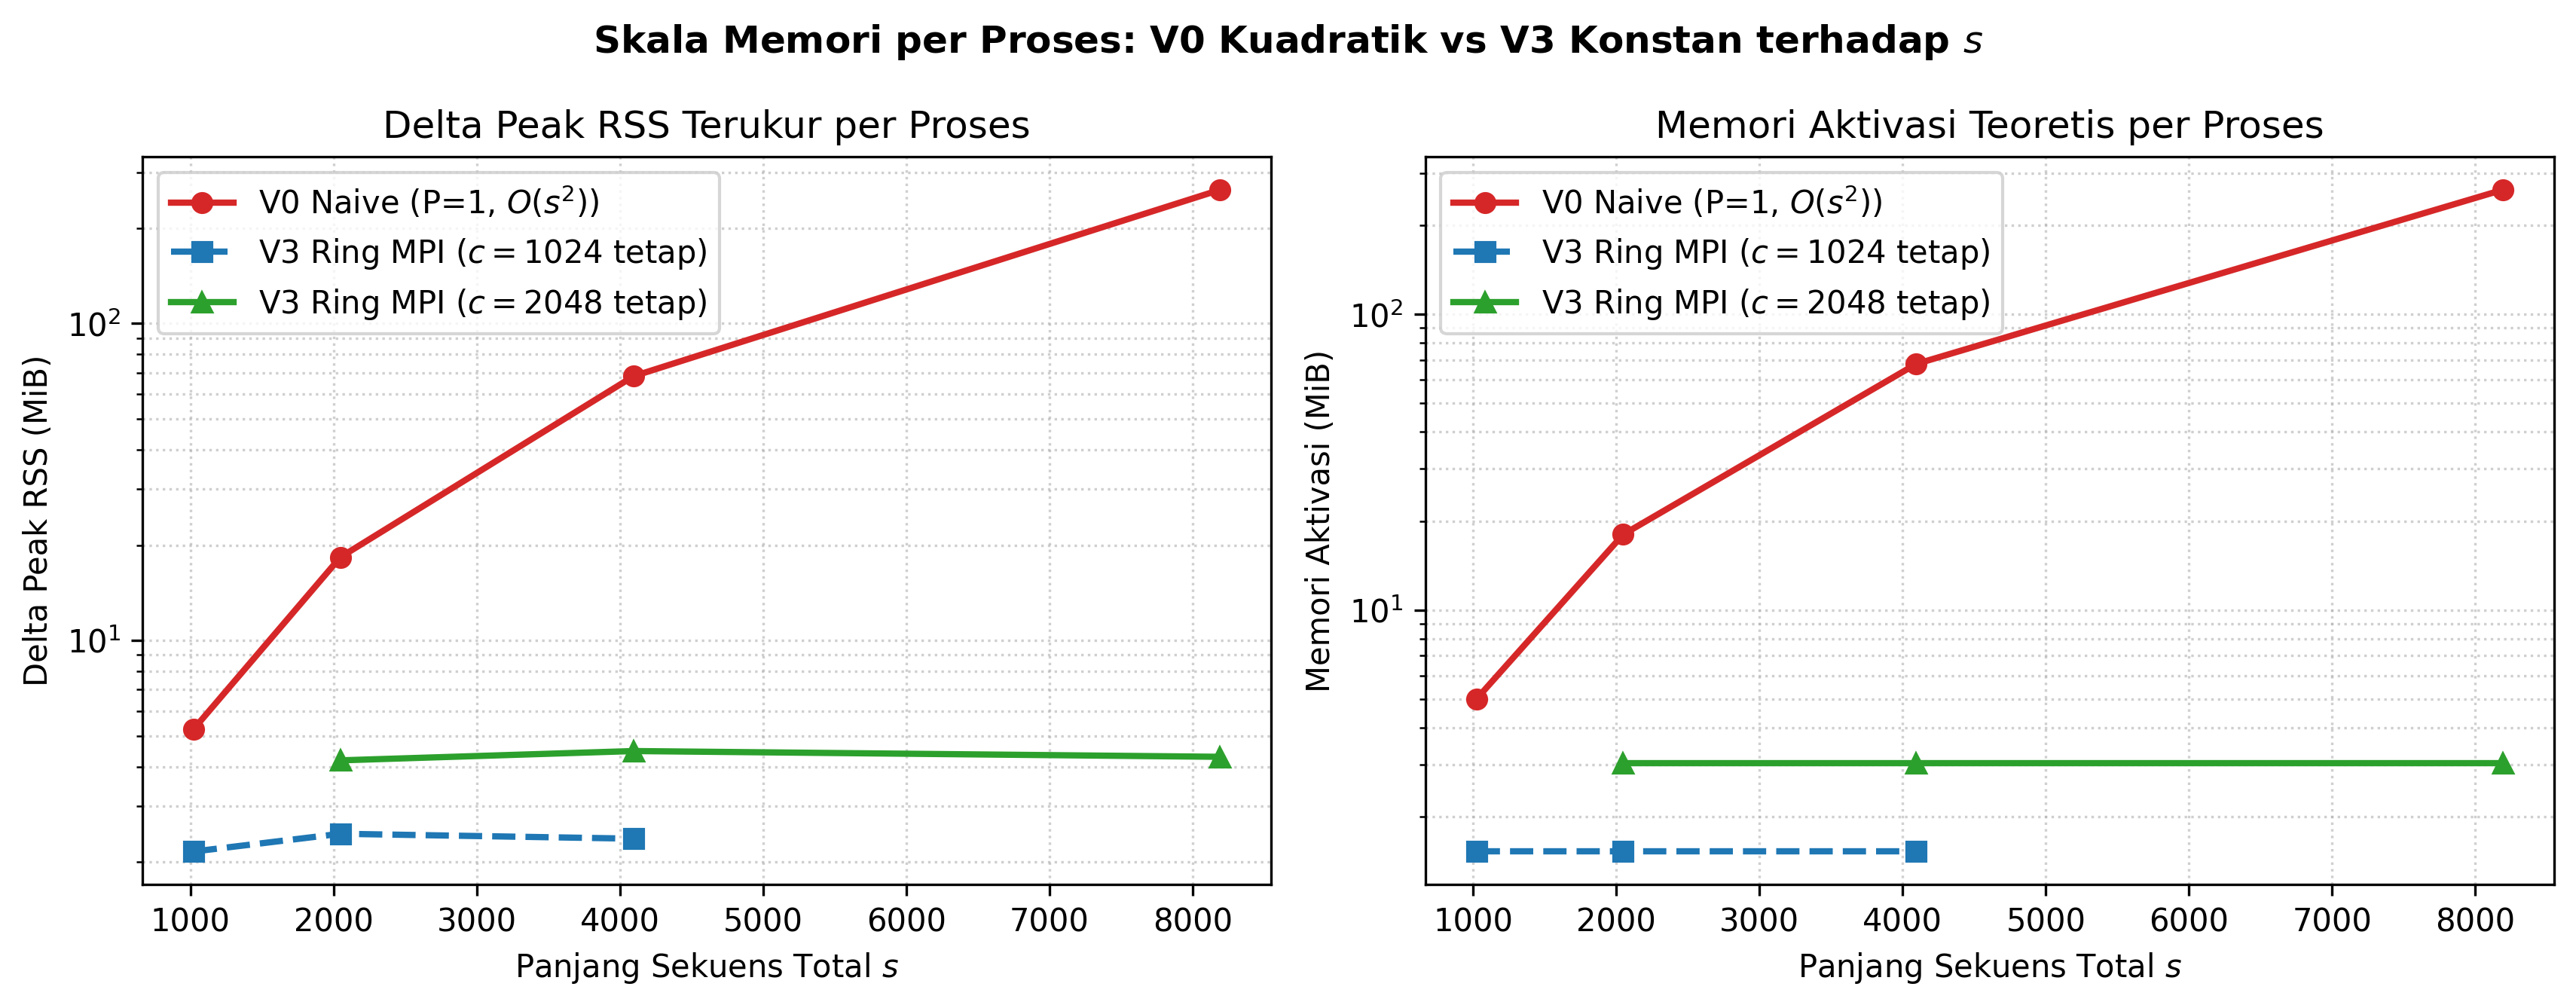
\includegraphics[width=0.96\textwidth]{../results/figures/01_memory_scaling_v0_vs_v3.png}
\caption{Skala memori per proses: pertumbuhan kuadratik V0 terhadap nilai konstan V3 pada ukuran blok $c$ tetap.}
\label{fig:mem}
\end{figure}

Pada $s=8192$, \emph{delta RSS} \textbf{V3} ($c=2048$) hanya \texttt{4.400 KiB}, yakni \textbf{61,5$\times$ lebih hemat} dibanding \textbf{V0} (\texttt{270.436 KiB}). Pada pengujian pembatasan memori \texttt{ulimit -v 1200000} KiB dengan $s=16384$ (\texttt{exp\_ulimit\_oom.csv}), \textbf{V0} ($P=1$) gagal dengan \texttt{std::bad\_alloc} (exit code 2), sedangkan \textbf{V3} ($P=4, c=4096$) berhasil selesai dalam \texttt{1.23435 s} dengan \texttt{peak\_rss\_kb = 184372} dan \texttt{delta\_rss\_kb = 11616}.

\subsection{Analisis Strong Scaling dan Weak Scaling}
Tabel~\ref{tab:strong} dan Gambar~\ref{fig:strong} menunjukkan performa \emph{strong scaling} pada $s=4096, d=64$ dari \texttt{v2\_strong\_scaling.csv} dan \texttt{exp\_strong\_scaling.csv}.

\begin{table}[H]
\centering
\caption{Hasil strong scaling V2 dan V3 pada $s=4096, d=64$.}
\label{tab:strong}
\begin{tabular}{lrrrrrrrrr}
\toprule
\textbf{Biner / Versi} & \textbf{$P$} & \textbf{$c$} & \textbf{Median (s)} & \textbf{Stddev (s)} & \textbf{GFLOP/s} & \textbf{Speedup} & \textbf{Efisiensi} & \textbf{Delta RSS (KiB)} \\
\midrule
\texttt{bench\_v2} (\texttt{v2}) & 1 & 256 & 0.261769 & 4.48e-03 & 16.407 & 1.000x & 100.0\% & --- \\
\texttt{bench\_v2} (\texttt{v2}) & 2 & 256 & 0.133798 & 3.52e-03 & 32.101 & 1.956x & 97.8\% & --- \\
\texttt{bench\_v2} (\texttt{v2}) & 4 & 256 & 0.074327 & 4.87e-03 & 57.785 & 3.522x & 88.0\% & --- \\
\texttt{attn} (\texttt{v2}) & 1 & 256 & 0.277894 & 1.13e-02 & 15.455 & 1.000x & 100.0\% & 4440 \\
\texttt{attn} (\texttt{v2}) & 2 & 256 & 0.128884 & 2.80e-03 & 33.324 & 2.156x & 107.8\% & 4396 \\
\texttt{attn} (\texttt{v2}) & 4 & 256 & 0.066261 & 3.19e-03 & 64.819 & 4.194x & 104.8\% & 4648 \\
\texttt{attn} (\texttt{v3}) & 1 & 4096 & 0.291810 & 7.55e-03 & 14.718 & 1.000x & 100.0\% & 8436 \\
\texttt{attn} (\texttt{v3}) & 2 & 2048 & 0.137857 & 1.84e-02 & 31.155 & 2.117x & 105.8\% & 4520 \\
\texttt{attn} (\texttt{v3}) & 4 & 1024 & 0.071210 & 1.45e-02 & 60.314 & 4.098x & 102.5\% & 2468 \\
\bottomrule
\end{tabular}
\end{table}

\begin{figure}[H]
\centering
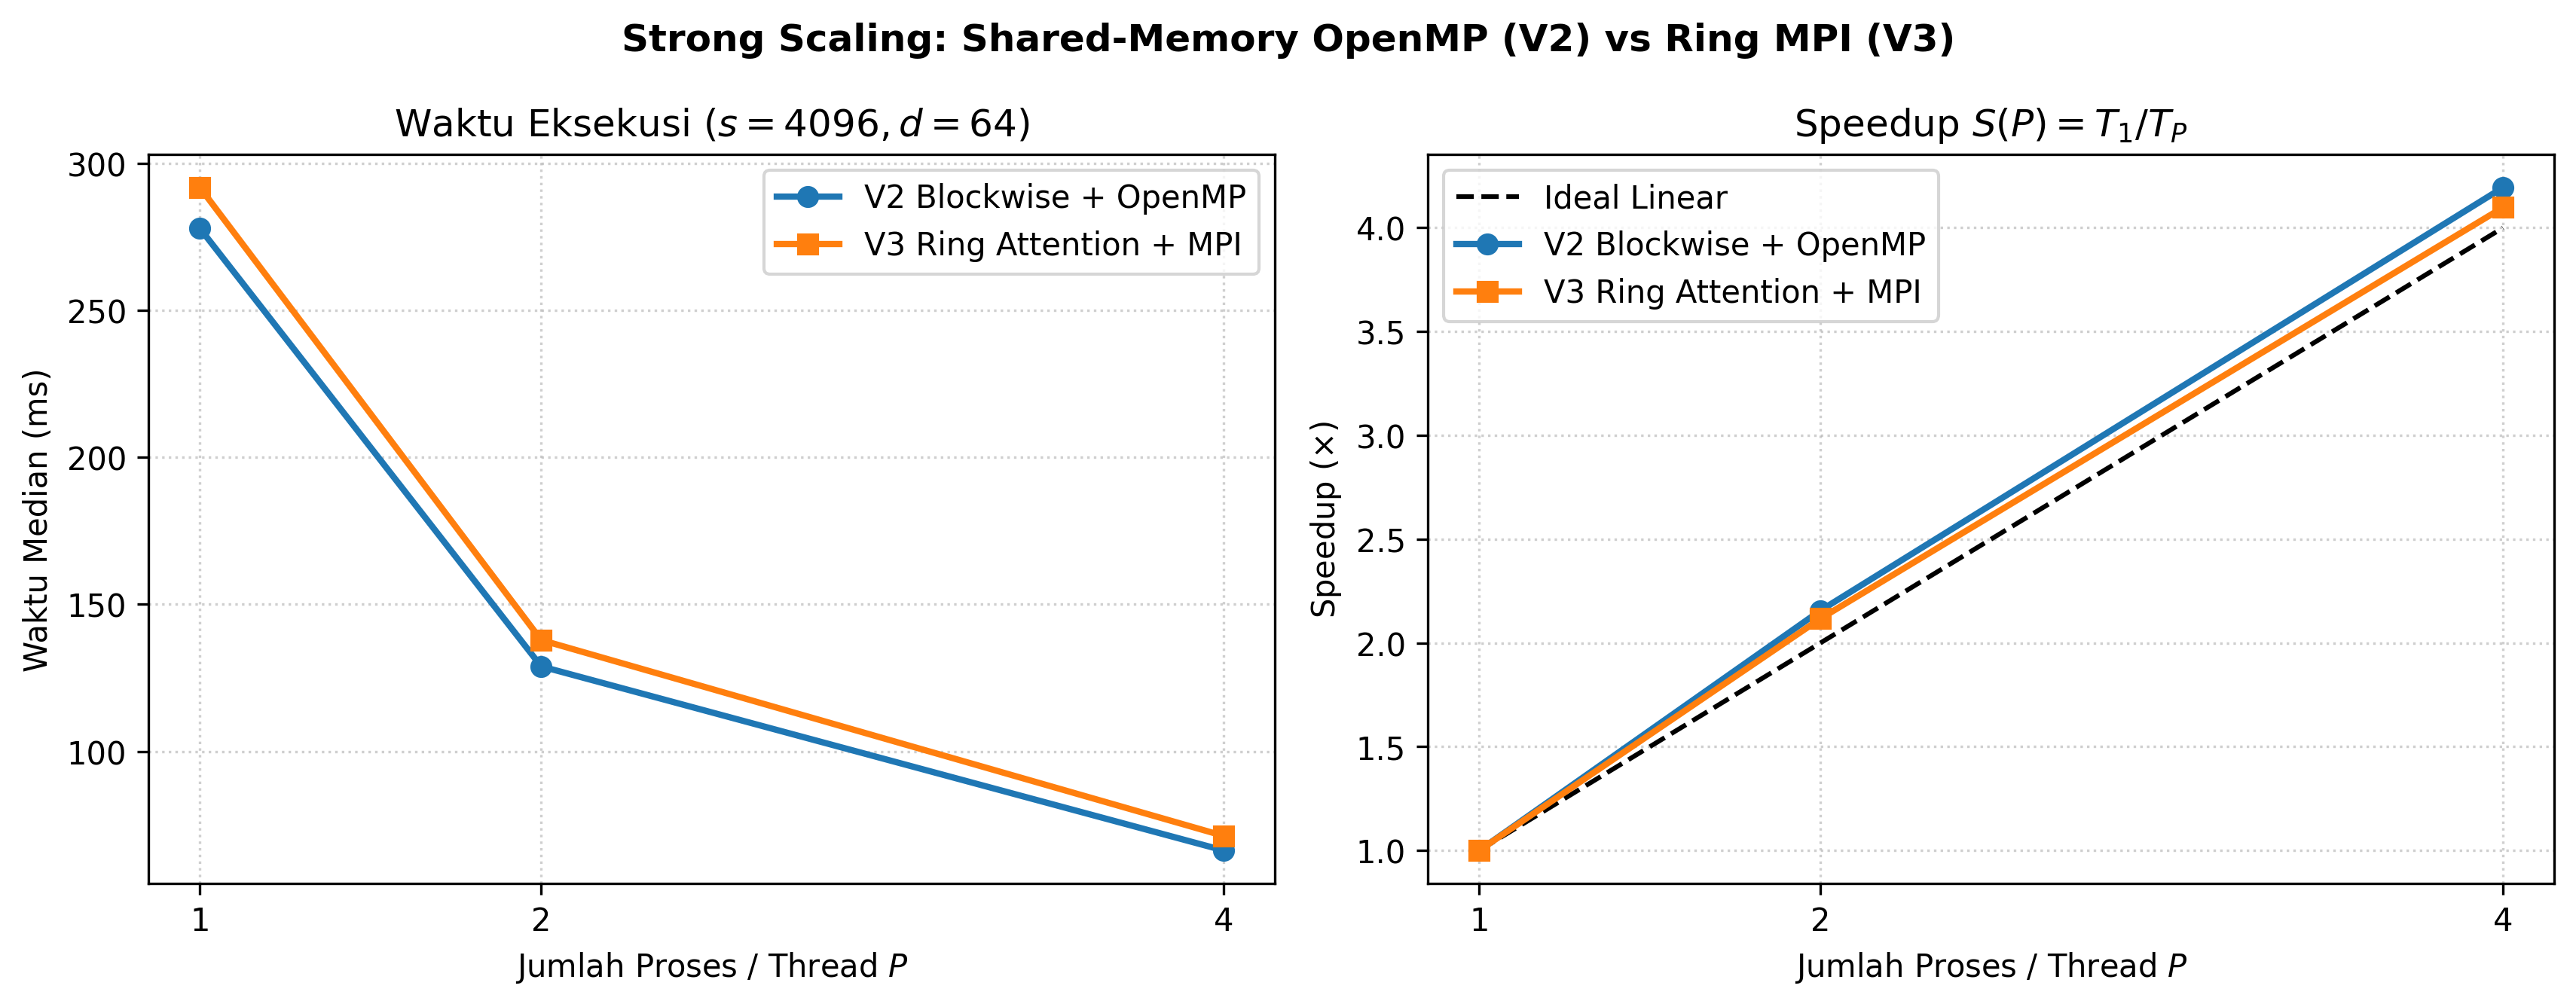
\includegraphics[width=0.96\textwidth]{../results/figures/02_strong_scaling.png}
\caption{Strong scaling V2 OpenMP dan V3 Ring MPI pada $s=4096, d=64$ ($P \in \{1, 2, 4\}$).}
\label{fig:strong}
\end{figure}

Profiling \texttt{/usr/bin/time -v} terhadap \texttt{bench\_v2\_scaling} mencatat \texttt{User time = 4.88 s}, \texttt{System time = 0.00 s}, dan \texttt{0} \emph{major page faults}, mengonfirmasi beban \emph{compute-bound} di ruang user. Gap antara laju attention $P=1$ (\texttt{14.7--16.4 GFLOP/s}) dan GEMM murni disebabkan oleh evaluasi skalar \texttt{std::exp()} per elemen tile $64\times 64$, sedangkan efisiensi $>100\%$ pada \texttt{attn} ($4.098\times$ untuk V3) terjadi karena penyusutan blok lokal $c=s/P$ sehingga lebih sesuai dengan cache L2/L3 serta variabilitas \emph{Turbo Boost} pada titik baseline $P=1$ (dibandingkan \texttt{bench\_v2\_scaling} mandiri yang mencatat $3.522\times$ / \texttt{88.0\%}).

Pada \emph{weak scaling} ($c=1024$ tetap, $s=P\cdot 1024$, Tabel~\ref{tab:weak} dan Gambar~\ref{fig:weak}), beban kerja per rank bertambah $P\times$ ($\mathcal{O}(Pc^2d)$) sementara memori aktivasi tetap konstan $\mathcal{O}(cd)$. Efisiensi skala kerja $(P\cdot T_1)/T_P$ pada \textbf{V3} mencapai \texttt{101.28\%} di $P=4$ (\texttt{63.963 GFLOP/s}), dengan anomali jitter sementara pada $P=2$ (\texttt{stddev = 6.87e-02 s}).

\begin{table}[H]
\centering
\caption{Hasil weak scaling pada $c = 1024$ tetap dan $s = P \cdot 1024$ (\texttt{exp\_weak\_scaling.csv}).}
\label{tab:weak}
\begin{tabular}{lrrrrrrrr}
\toprule
\textbf{Versi} & \textbf{$P$} & \textbf{$s$} & \textbf{Median (s)} & \textbf{Stddev (s)} & \textbf{Total GFLOP/s} & \textbf{GFLOP/s/Proc} & \textbf{Work Eff} & \textbf{Delta RSS (KiB)} \\
\midrule
\texttt{v2} & 1 & 1024 & 1.719080e-02 & 6.26e-03 & 15.615 & 15.615 & 100.00\% & 1292 \\
\texttt{v2} & 2 & 2048 & 3.325604e-02 & 3.20e-03 & 32.287 & 16.144 & 103.38\% & 2396 \\
\texttt{v2} & 4 & 4096 & 6.610271e-02 & 1.55e-03 & 64.974 & 16.244 & 104.02\% & 4544 \\
\texttt{v3} & 1 & 1024 & 1.700211e-02 & 8.32e-03 & 15.788 & 15.788 & 100.00\% & 2304 \\
\texttt{v3} & 2 & 2048 & 6.011445e-02 & 6.87e-02 & 17.862 & 8.931 & 56.57\% & 2532 \\
\texttt{v3} & 4 & 4096 & 6.714810e-02 & 2.00e-02 & 63.963 & 15.991 & 101.28\% & 2488 \\
\bottomrule
\end{tabular}
\end{table}

\begin{figure}[H]
\centering
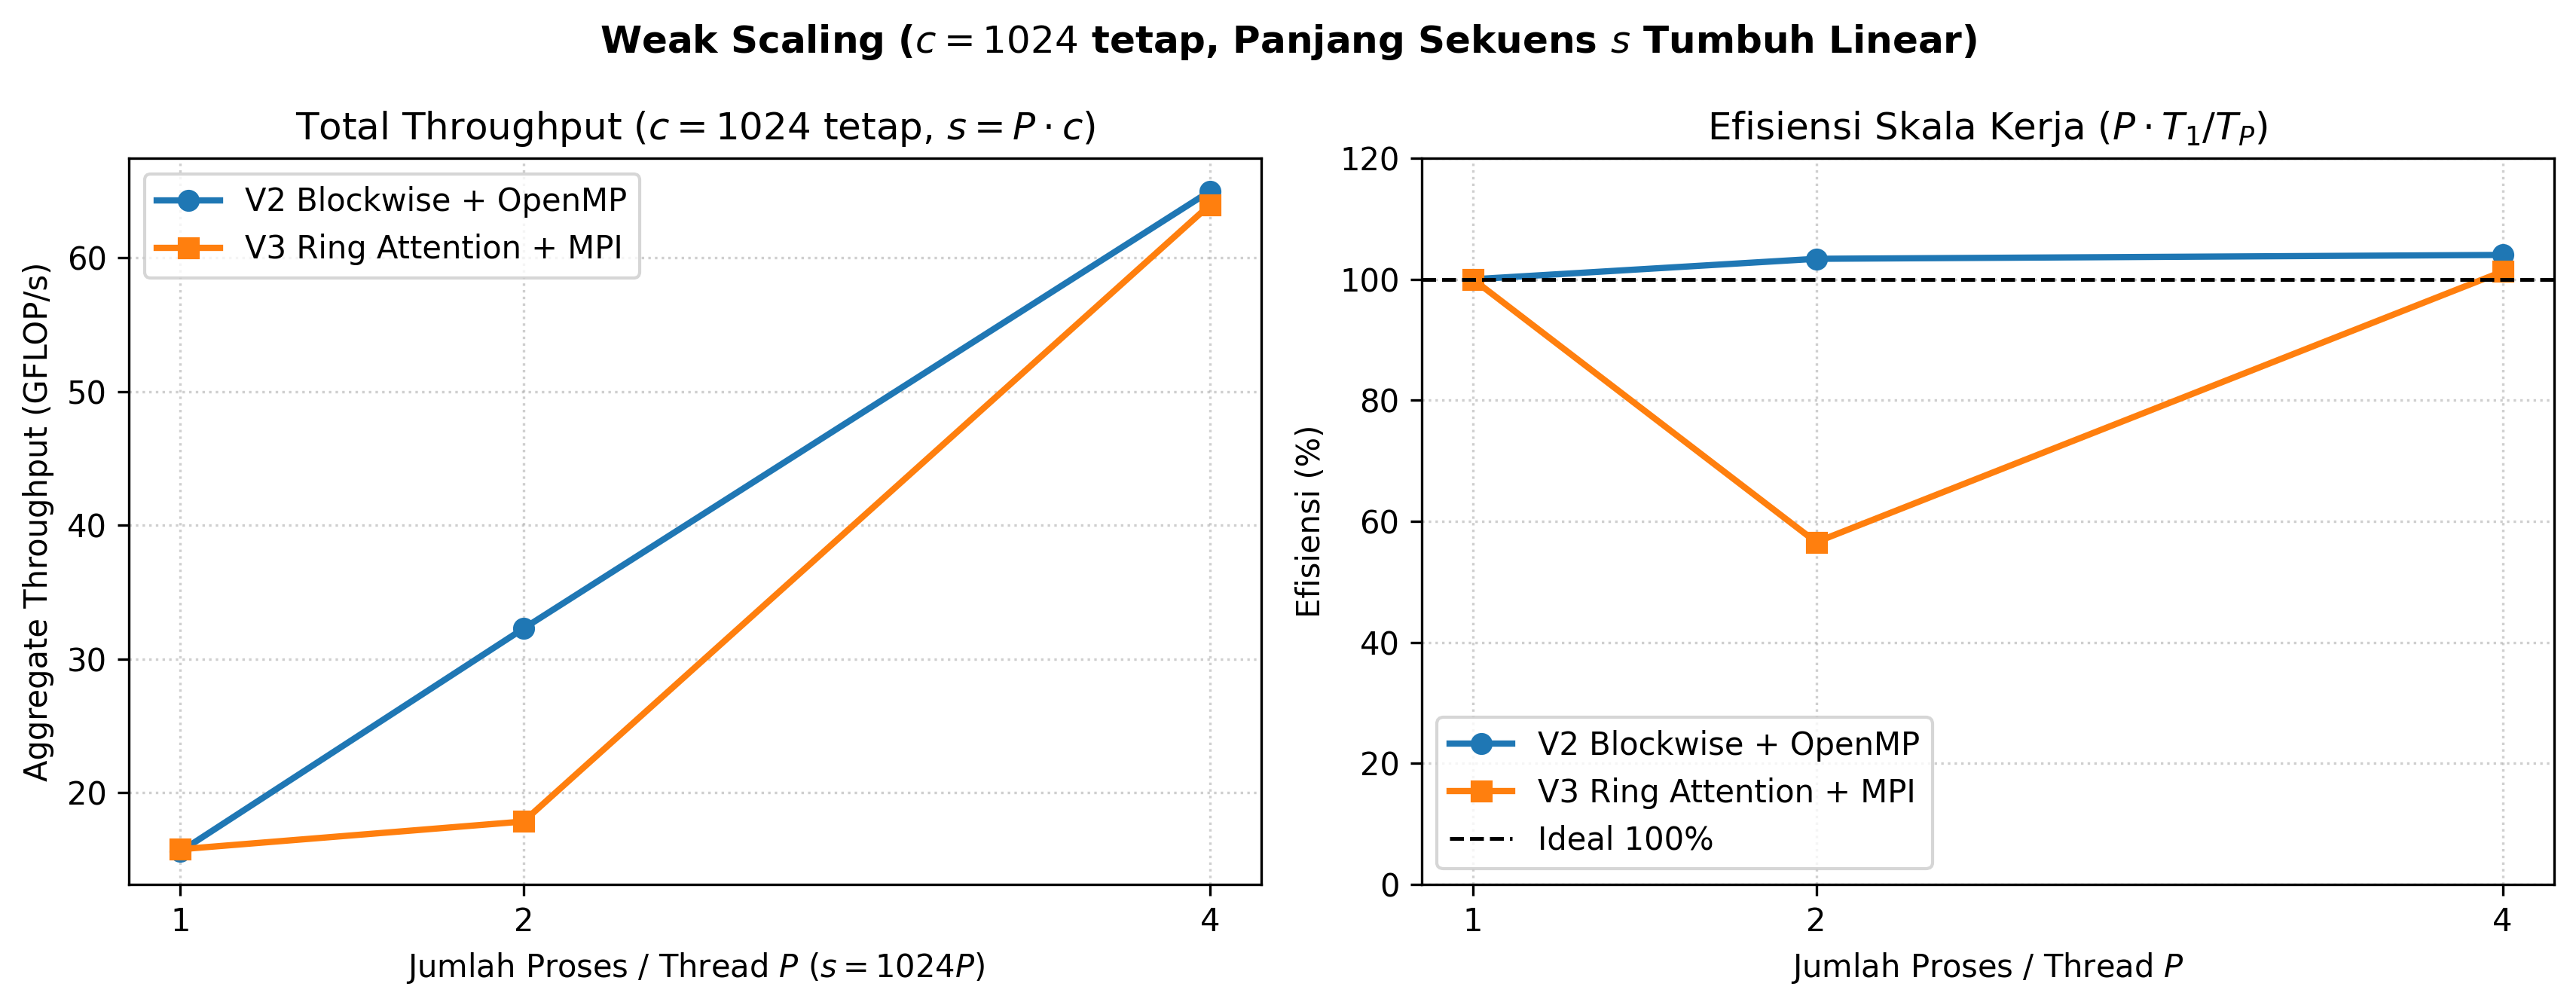
\includegraphics[width=0.96\textwidth]{../results/figures/03_weak_scaling.png}
\caption{Throughput agregat dan efisiensi skala kerja pada weak scaling ($c=1024$ tetap).}
\label{fig:weak}
\end{figure}

\subsection{Efektivitas Overlap (\texorpdfstring{$\eta$}{eta}) dan Validasi Model Analitik (\texorpdfstring{$c \ge 2F/B$}{c >= 2F/B})}
Mikro-benchmark GEMM (\texttt{gemm\_benchmark.csv}) pada 1 core mengukur laju $F$ sebesar \texttt{33.994 GFLOP/s} (\texttt{NT}) dan \texttt{42.217 GFLOP/s} (\texttt{NN}) di ukuran tile $64\times 64\times 64$ (rerata $38.11\text{ GFLOP/s}$), hingga \texttt{47.795 GFLOP/s} pada $512\times 512\times 128$. Sementara mikro-benchmark ping-pong OpenMPI (\texttt{mpi\_pingpong.csv}) mencatat latensi 64 B sebesar \texttt{1.020 $\mu$s} serta bandwidth $B$ sebesar \texttt{1.9917}, \texttt{2.2284}, \texttt{2.3926}, \texttt{2.8894}, dan \texttt{2.9425 GB/s} untuk ukuran payload $[K|V]$ pada $c=128, 256, 512, 1024, 2048$ (melonjak ke \texttt{7.3047 GB/s} pada $2\text{ MiB}$).

\begin{table}[H]
\centering
\caption{Efektivitas overlap komunikasi--komputasi V3 ($P=4, d=64$) dan prediksi model $c \ge 2F/B$ (\texttt{exp\_overlap.csv}).}
\label{tab:overlap}
\begin{tabular}{rrrrrrrrrr}
\toprule
\textbf{$c$} & \textbf{$s$} & \textbf{$T_{\mathrm{blk}}$ (s)} & \textbf{$T_{\mathrm{nb}}$ (s)} & \textbf{$T_{\mathrm{comp}}$ (s)} & \textbf{$T_{\mathrm{wait}}$ (s)} & \textbf{$\eta$} & \textbf{$B$ (GB/s)} & \textbf{$c_{\min}$ (GEMM)} & \textbf{$c_{\min}$ (Attn)} \\
\midrule
128 & 512 & 3.286e-03 & 4.643e-03 & 2.770e-03 & 9.035e-04 & -2.6285 & 1.992 & 38.3 & 6.1 \\
256 & 1024 & 1.171e-02 & 1.149e-02 & 1.117e-02 & 2.945e-04 & 0.4112 & 2.228 & 34.2 & 5.4 \\
512 & 2048 & 4.474e-02 & 4.451e-02 & 4.016e-02 & 2.575e-04 & 0.0500 & 2.393 & 31.9 & 5.6 \\
1024 & 4096 & 6.809e-02 & 7.085e-02 & 6.681e-02 & 6.587e-03 & -2.1509 & 2.889 & 26.4 & 11.1 \\
2048 & 8192 & 2.794e-01 & 2.744e-01 & 2.732e-01 & 4.855e-03 & \textbf{0.8106} & 2.942 & 25.9 & 10.7 \\
\bottomrule
\end{tabular}
\end{table}

\begin{figure}[H]
\centering
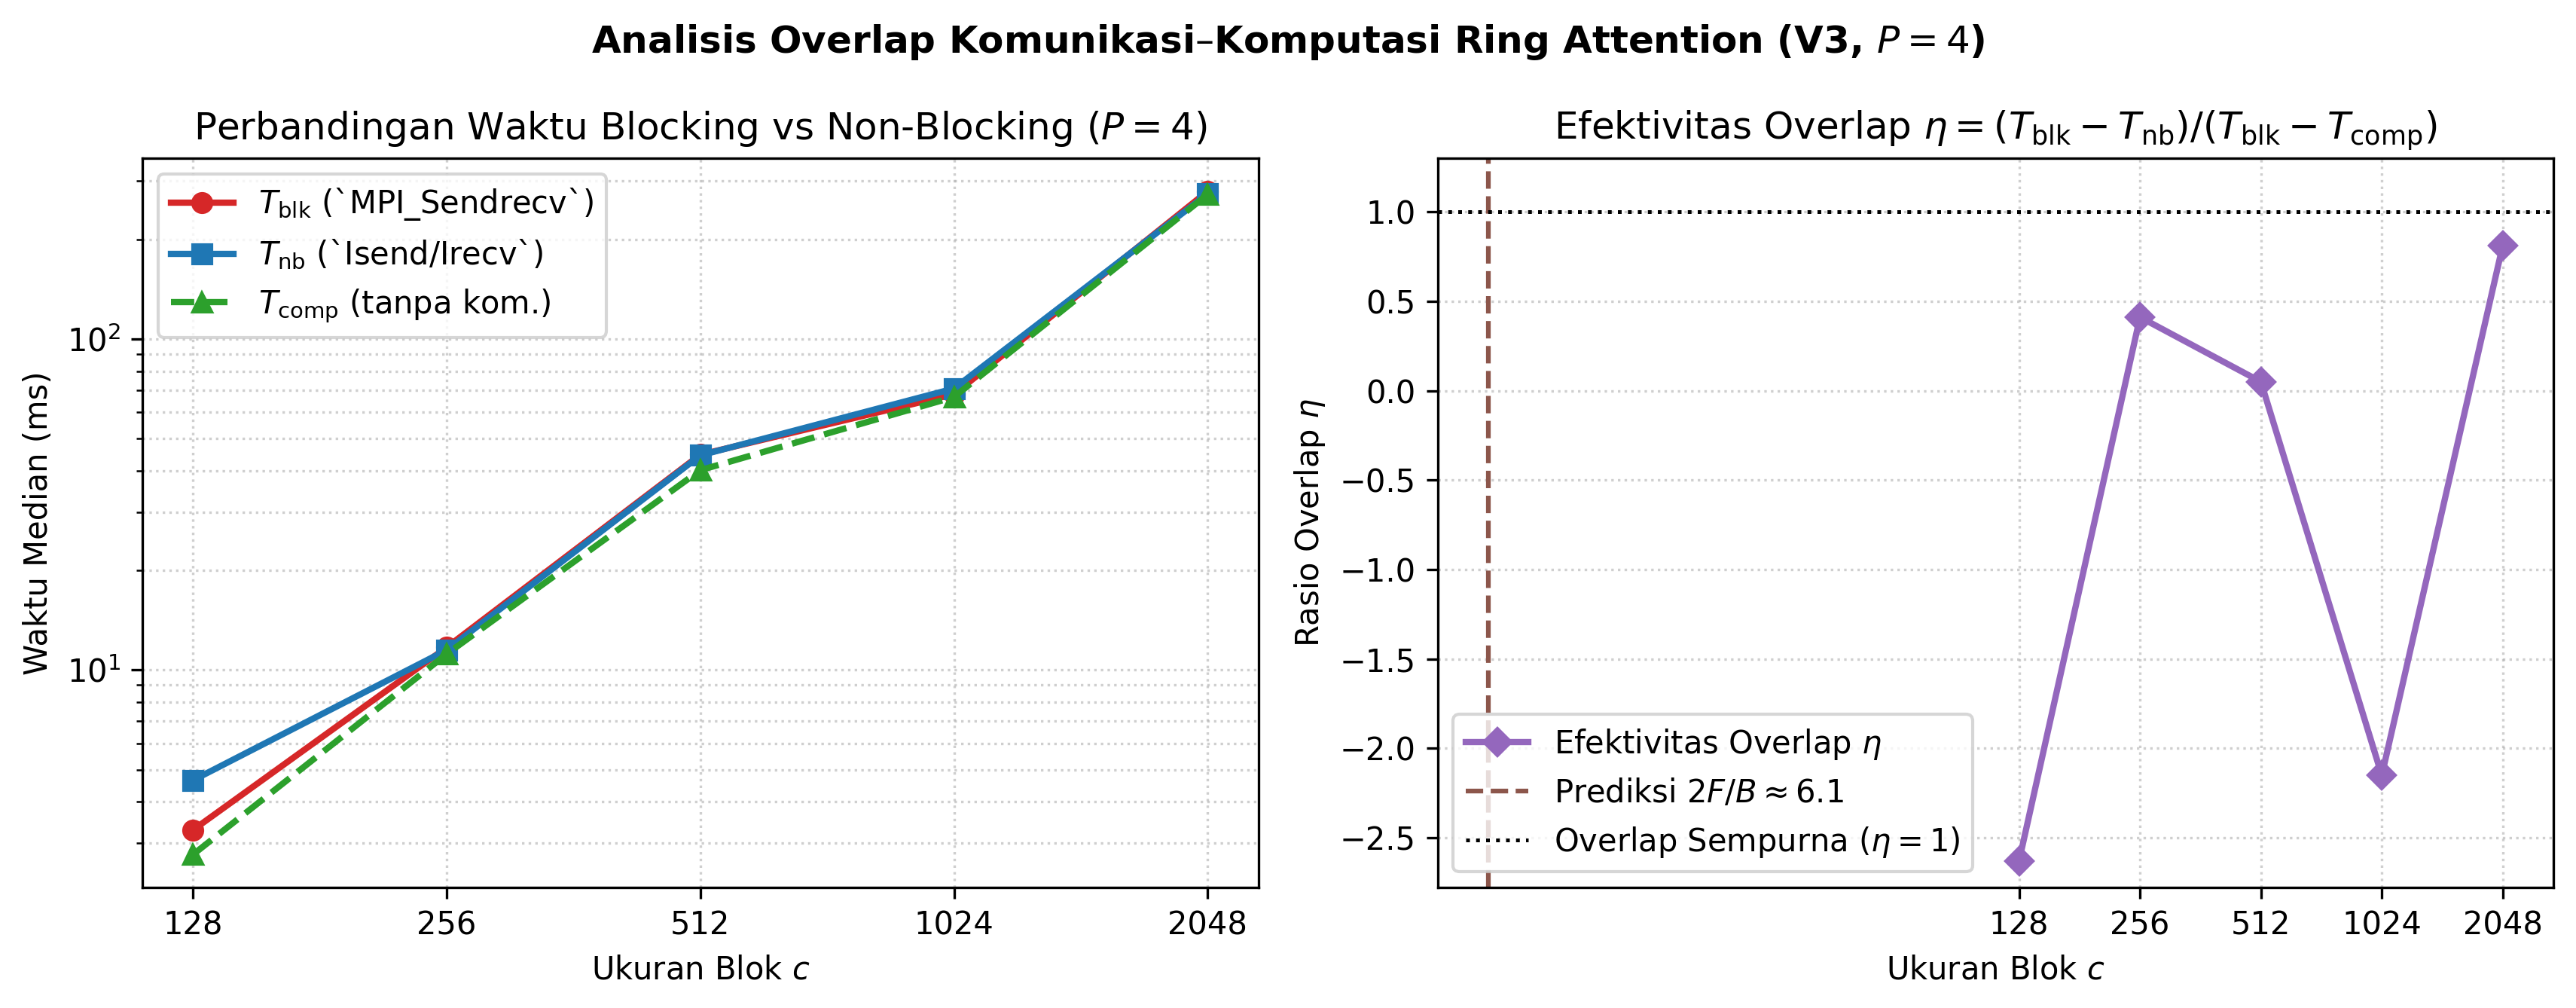
\includegraphics[width=0.96\textwidth]{../results/figures/04_overlap_analysis.png}
\caption{Perbandingan $T_{\mathrm{blk}}$, $T_{\mathrm{nb}}$, $T_{\mathrm{comp}}$ dan rasio efektivitas overlap $\eta$ terhadap $c$.}
\label{fig:overlap}
\end{figure}

Secara analitik, $c_{\min} = 2F/B \in [25.9, 38.3]$ (untuk $F_{\mathrm{GEMM}}$) menunjukkan bahwa $c \ge 128$ secara teori cukup untuk menyembunyikan transfer. Pada praktik mesin tunggal (\emph{shared-memory}), ketika $c \le 1024$ selisih $T_{\mathrm{blk}} - T_{\mathrm{comp}}$ hanya $0.5$--$4.6\text{ ms}$ sehingga ketiadaan progres latar OpenMPI sampai \texttt{MPI\_Waitall} serta perebutan bandwidth memori memunculkan jitter yang membuat $\eta$ berfluktuasi. Ketika durasi komputasi membesar di $c = 2048$ ($273.2\text{ ms}$), biaya tunggu \texttt{MPI\_Waitall} tinggal $4.85\text{ ms}$ ($1.77\%$) dan efektivitas overlap mencapai \textbf{$\eta = 0.8106$}.

\subsection{Evaluasi Aplikasi Triase DNA Payudara (Sebelum vs Sesudah)}
Model \texttt{BreastTriageTransformer} mencatat metrik sekunder pelatihan offline \texttt{val\_accuracy = 1.0}, \texttt{val\_f1 = 1.0}, dan \texttt{leave\_one\_line\_out\_184AA2\_acc = 1.0}. Tabel~\ref{tab:app} dan Gambar~\ref{fig:app} menampilkan evaluasi end-to-end antara \textbf{V0} dan \textbf{V3} ($P=4$) dari \texttt{exp\_app\_comparison.csv}.

\begin{table}[H]
\centering
\caption{Perbandingan aplikasi triase DNA sebelum (V0) dan sesudah optimasi (V3, $P=4$) (\texttt{exp\_app\_comparison.csv}).}
\label{tab:app}
\begin{tabular}{lrlrrrrr}
\toprule
\textbf{Sampel} & \textbf{$s$} & \textbf{Versi} & \textbf{Waktu (s)} & \textbf{Stddev (s)} & \textbf{Throughput (read/s)} & \textbf{Peak RSS (KiB)} & \textbf{Delta RSS (KiB)} \\
\midrule
\texttt{184D\_normal} & 1024 & \texttt{v0} ($P=1$) & 4.712e-02 & 5.68e-03 & 869.24 & 179668 & 7028 \\
\texttt{184D\_normal} & 1024 & \texttt{v3} ($P=4$) & 1.283e-02 & 2.46e-03 & 3191.76 & 174900 & 2088 \\
\texttt{184D\_normal} & 2048 & \texttt{v0} ($P=1$) & 1.454e-01 & 1.63e-03 & 563.51 & 193520 & 20792 \\
\texttt{184D\_normal} & 2048 & \texttt{v3} ($P=4$) & 4.595e-02 & 1.25e-02 & 1782.64 & 175588 & 2764 \\
\texttt{184D\_normal} & 4096 & \texttt{v0} ($P=1$) & 3.719e-01 & 1.37e-02 & 440.49 & 245812 & 73076 \\
\texttt{184D\_normal} & 4096 & \texttt{v3} ($P=4$) & 1.101e-01 & 4.67e-02 & 1487.88 & 176792 & 4076 \\
\texttt{184D\_normal} & 8192 & \texttt{v0} ($P=1$) & 1.219e+00 & 2.47e-02 & 268.73 & 448376 & 275736 \\
\texttt{184D\_normal} & 8192 & \texttt{v3} ($P=4$) & 4.148e-01 & 1.96e-03 & 790.04 & 179380 & 6528 \\
\midrule
\texttt{184AA2\_aig} & 1024 & \texttt{v0} ($P=1$) & 4.322e-02 & 3.33e-03 & 947.81 & 179620 & 6952 \\
\texttt{184AA2\_aig} & 1024 & \texttt{v3} ($P=4$) & 1.261e-02 & 2.74e-03 & 3248.73 & 174904 & 2080 \\
\texttt{184AA2\_aig} & 2048 & \texttt{v0} ($P=1$) & 1.403e-01 & 9.91e-03 & 584.03 & 193512 & 20872 \\
\texttt{184AA2\_aig} & 2048 & \texttt{v3} ($P=4$) & 4.664e-02 & 7.64e-03 & 1756.45 & 175568 & 2732 \\
\texttt{184AA2\_aig} & 4096 & \texttt{v0} ($P=1$) & 3.992e-01 & 1.25e-02 & 410.40 & 245616 & 72964 \\
\texttt{184AA2\_aig} & 4096 & \texttt{v3} ($P=4$) & 1.782e-01 & 1.18e-02 & 919.62 & 176896 & 3996 \\
\texttt{184AA2\_aig} & 8192 & \texttt{v0} ($P=1$) & 1.344e+00 & 7.36e-02 & 243.86 & 448580 & 275864 \\
\texttt{184AA2\_aig} & 8192 & \texttt{v3} ($P=4$) & 4.244e-01 & 1.02e-02 & 772.15 & 179456 & 6496 \\
\bottomrule
\end{tabular}
\end{table}

\begin{figure}[H]
\centering
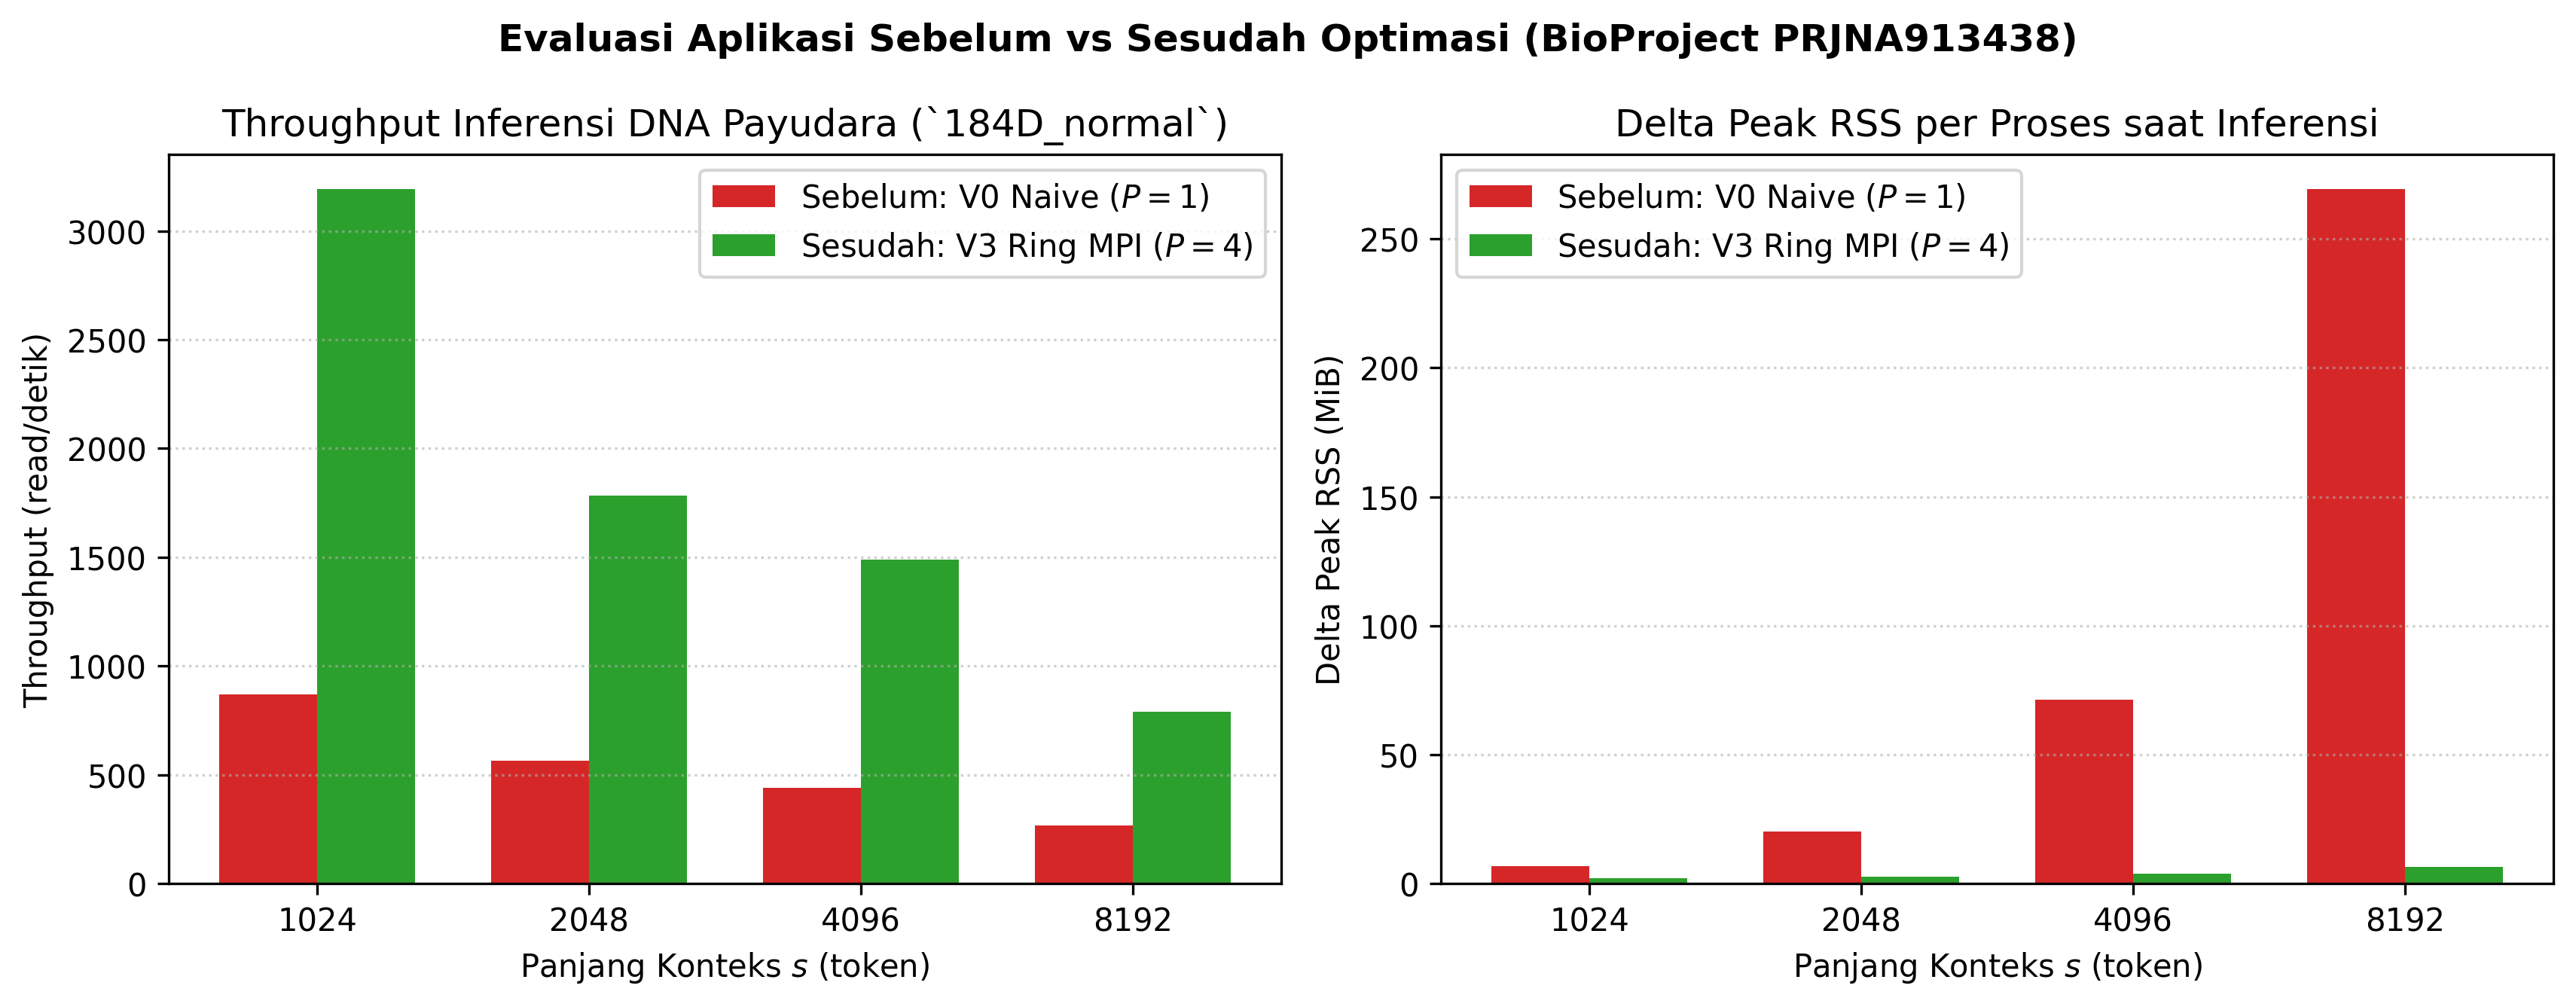
\includegraphics[width=0.96\textwidth]{../results/figures/05_app_before_after_dna.png}
\caption{Evaluasi aplikasi triase DNA sebelum (V0) dan sesudah optimasi (V3, $P=4$) pada sampel \texttt{184D\_normal}.}
\label{fig:app}
\end{figure}

Seluruh prediksi pada kedua sampel mencapai keyakinan \texttt{100.00\%} (\texttt{Normal-like} untuk \texttt{184D\_normal} dan \texttt{Progresi Karsinogenesis} untuk \texttt{184AA2\_aig}). Pada $s=8192$, \textbf{V3} mempercepat waktu inferensi sebesar \textbf{2.94$\times$}--\textbf{3.17$\times$} (\texttt{790.04} dan \texttt{772.15 read/detik}) dan menekan \emph{delta RSS} sebesar \textbf{42.2$\times$}--\textbf{42.5$\times$}.

\section{Kesimpulan, Keterbatasan, dan Pengembangan Lanjutan}

\subsection{Kesimpulan}
Seluruh luaran wajib dan opsional proyek telah tervalidasi: (1) seluruh versi V1--V4 lolos toleransi numerik $< 10^{-5}$ terhadap V0-FP64 (\texttt{rel\_err} $\le 1.227\times 10^{-6}$); (2) memori aktivasi per proses V3 terbukti konstan $\mathcal{O}(cd)$ terhadap $s$ serta tetap berjalan pada $s=16384$ di bawah \texttt{ulimit -v 1200000} saat V0 gagal OOM; (3) strong scaling mencapai speedup \texttt{4.194x} (V2) dan \texttt{4.098x} (V3) pada 4 core fisik dengan overlap $\eta = 0.8106$ di $c=2048$; dan (4) integrasi triase DNA payudara menunjukkan percepatan hingga \texttt{3.17x} dan penghematan memori aktivasi $> 42\times$.

\subsection{Keterbatasan dan Pengembangan Lanjutan}
Keterbatasan utama meliputi emulasi pada satu mesin \emph{shared-memory} (berbeda dari interkoneksi klaster InfiniBand/NVLink), pembatasan \texttt{perf\_event\_paranoid=4} pada host, serta penggunaan subset FASTQ sintetis offline dengan satu lini kontrol normal. Pengembangan lanjutan mencakup eksekusi MPI multi-node melalui \emph{hostfile}, vektorisasi SIMD untuk operasi \texttt{expf()}, dukungan \emph{multi-head attention} serta \emph{backward pass}, dan validasi klinis pada data kohort pasien nyata.

\begin{thebibliography}{11}
\bibitem{liu2023ring} H. Liu, M. Zaharia, \& P. Abbeel. \emph{Ring Attention with Blockwise Transformers for Near-Infinite Context}. arXiv:2310.01889, 2023.
\bibitem{liu2023bpt} H. Liu \& P. Abbeel. \emph{Blockwise Parallel Transformer for Large Context Models}. NeurIPS, 2023.
\bibitem{dao2022} T. Dao, D. Fu, S. Ermon, A. Rudra, \& C. R\'e. \emph{FlashAttention: Fast and Memory-Efficient Exact Attention with IO-Awareness}. NeurIPS, 2022.
\bibitem{rabe2021} M. N. Rabe \& C. Staats. \emph{Self-attention Does Not Need $O(n^2)$ Memory}. arXiv:2112.05682, 2021.
\bibitem{milakov2018} M. Milakov \& N. Gimelshein. \emph{Online Normalizer Calculation for Softmax}. arXiv:1805.02867, 2018.
\bibitem{li2023} S. Li, F. Xue, C. Baranwal, Y. Li, \& Y. You. \emph{Sequence Parallelism: Long Sequence Training from System Perspective}. ACL, 2023.
\bibitem{jacobs2023} S. A. Jacobs dkk. \emph{DeepSpeed Ulysses: System Optimizations for Enabling Training of Extreme Long Sequence Transformer Models}. arXiv:2309.14509, 2023.
\bibitem{vaswani2017} A. Vaswani dkk. \emph{Attention Is All You Need}. NeurIPS, 2017.
\bibitem{park2023} J.-L. Park, J.-Y. Kim, S.-Y. Kim, \& Y. S. Lee. \emph{Generation and analysis of whole-genome sequencing data in human mammary epithelial cells}. Genomics \& Informatics, 2023 (PRJNA913438).
\bibitem{nguyen2023} E. Nguyen dkk. \emph{HyenaDNA: Long-Range Genomic Sequence Modeling at Single Nucleotide Resolution}. NeurIPS, 2023.
\bibitem{ji2021} Y. Ji, Z. Zhou, H. Liu, \& R. V. Davuluri. \emph{DNABERT: pre-trained Bidirectional Encoder Representations from Transformers model for DNA-language in genome}. Bioinformatics, 37(15):2112--2120, 2021.
\end{thebibliography}

\end{document}
